\documentclass[12pt,letterpaper]{article}

\usepackage[spanish,es-tabla,es-nodecimaldot]{babel}
\usepackage{amsmath}
\usepackage[utf8]{inputenc}
\usepackage[T1]{fontenc}
\usepackage{lmodern}
\usepackage{graphicx}
\usepackage{listings}
\usepackage{anysize} 
\usepackage{fancyhdr}
\usepackage{amsmath}
\usepackage{pdfpages}
\usepackage{graphics}
\usepackage{capt-of}
\usepackage{tabularx}
\usepackage[colorlinks=true,plainpages=true,citecolor=blue,linkcolor=blue]{hyperref}

\marginsize{2cm}{2cm}{2cm}{2cm}
\pagestyle{fancy}
\fancyhf{Líneas de transmisión y antenas}
\fancyhead[L]{\footnotesize UPIITA-IPN} 
\fancyhead[R]{\footnotesize 3TV1} 
\fancyfoot[R]{\footnotesize Práctica 2}
\fancyfoot[C]{\thepage}
\fancyfoot[L]{\footnotesize Patrones de radiación} 

\renewcommand{\footrulewidth}{0.4pt}
\renewcommand{\spanishtablename}{Tabla}
\renewcommand{\labelitemii}{$\star$}

\begin{document}


\includepdf[pages={1}]{portada}

\newpage
\tableofcontents
%\listoffigures
%\listoftables

\newpage
\section{Antecedentes}
\subsection{Antenas de dipolo}
En radio y telecomunicaciones una antena de dipolo es la clase de antena más 
simple y más utilizada. Una antena de dipolo suele estar formada por dos 
elementos conductores idénticos, como alambres o varillas metálicas. Se aplica 
la corriente de accionamiento del transmisor o, para las antenas de recepción, se toma la 
señal de salida al receptor, entre las dos mitades de la antena. Cada lado de la línea 
de alimentación al transmisor o receptor está conectado a uno de los conductores.
\\ \\
Más comúnmente consiste en dos conductores de igual longitud orientados de extremo a 
extremo con la línea de alimentación conectada entre ellos. Los dipolos se utilizan 
frecuentemente como antenas resonantes. El uso de la antena alrededor de esa 
frecuencia es ventajoso en términos de impedancia del punto de alimentación (y por lo tanto 
de relación de onda estacionaria), por lo que su longitud está determinada por la longitud 
de onda prevista (o frecuencia) de operación. El más comúnmente utilizado es el dipolo 
de media onda alimentado por el centro, que es justo por debajo de una media longitud de 
onda. 
\\ \\
Algunos tipos comunes de antenas de dipolo son:
\begin{itemize}
    \item Antena dipolo de media onda.
    \item Antena dipolo plegada o doblado.
\end{itemize}

\subsection{Antena de dipolo de media onda}
El dipolo de media onda está formado por un elemento conductor que es un alambre o un tubo de 
metal que es de media longitud de onda eléctrica de largo. El dipolo de media onda se 
alimenta normalmente en el centro, donde la impedancia cae a su nivel más bajo. De esta 
manera, la antena consiste en el alimentador conectado a dos elementos de cuarto de 
longitud de onda alineados entre sí.
\\
\begin{figure}[ht]
    \centering
    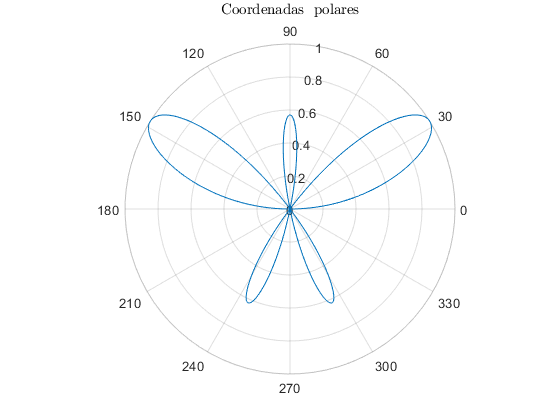
\includegraphics[width=.4\textwidth]{f3.png}
    \caption{Antena de dipolo.}
\end{figure}
\\
Debe recordarse que la longitud del dipolo de media onda es una media longitud de onda 
eléctrica para la onda que viaja en los conductores de la antena. Esto es ligeramente 
más corto que la longitud equivalente de una onda que viaja en el espacio libre, ya que 
los conductores de la antena afectan a la longitud de onda.

\subsubsection{Patron de radianción}
\begin{figure}[ht]
    \centering
    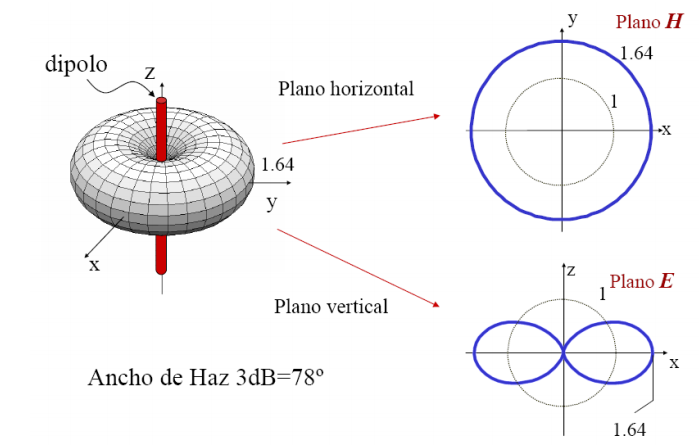
\includegraphics[width=.7\textwidth]{fig1.png}
    \caption{Patron de radiación de dipolo sencillo.}
\end{figure}
Patrón de radiación para diferenetes longitudes de onda.
\begin{figure}[ht]
    \centering
    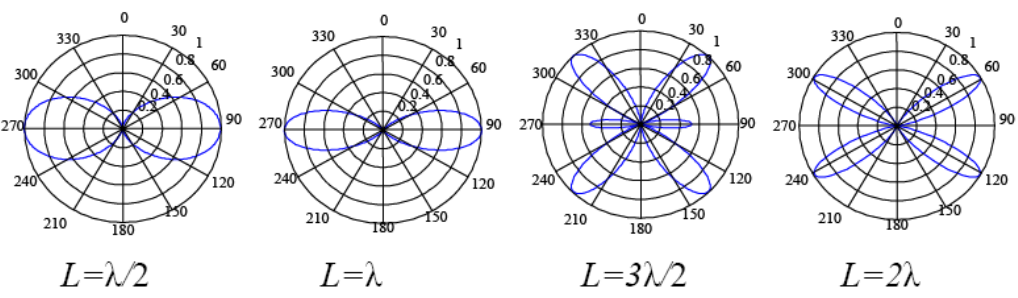
\includegraphics[width=1\textwidth]{fig2.png}
    \caption{Patrones de radiación para diferenetes longitudes de onda y longitudes fisicas.}
\end{figure}

\newpage
\subsection{Antena de dipolo doblado}
Un dipolo doblado es una estructura formada por dos dipolos
paralelos, cortocircuitados en su extremo. Uno de ellos se alimenta
en el centro con un generador.
El dipolo doblado se puede descomponer en el modo par o modo
antena, con la misma alimentación en los dos brazos, y el modo
impar o modo línea de transmisión, con dos generadores con signos
opuestos.
\begin{figure}[ht]
    \centering
    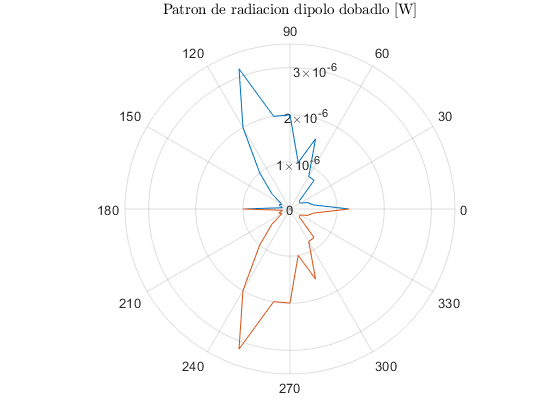
\includegraphics[width=.4\textwidth]{f5.png}
    \caption{Dipolo doblado.}
\end{figure}
\\
\textbf{Ventajas de un dipolo doblado}
\\
Hay dos ventajas principales para el uso de una antena dipolo plegada sobre un dipolo estándar:
\begin{itemize}
    \item Aumento de la impedancia:   Cuando es necesario utilizar alimentadores de alta impedancia, 
    o cuando la impedancia del dipolo se reduce por factores tales como elementos parasitarios, 
    un dipolo plegado proporciona un aumento significativo en el nivel de impedancia que permite 
    que la antena se adapte más fácilmente al alimentador disponible.
    \item Ancho de banda amplio: La antena dipolo plegada tiene una respuesta de frecuencia más plana - 
    esto permite que se utilice sobre un ancho de banda más amplio con muchas transmisiones que 
    utilizan una variedad de diferentes canales seleccionables, por ejemplo, televisión y radio 
    de difusión, se necesita una antena de ancho de banda amplio.
\end{itemize}

\subsubsection{Patron de radianción}
\begin{figure}[ht]
    \centering
    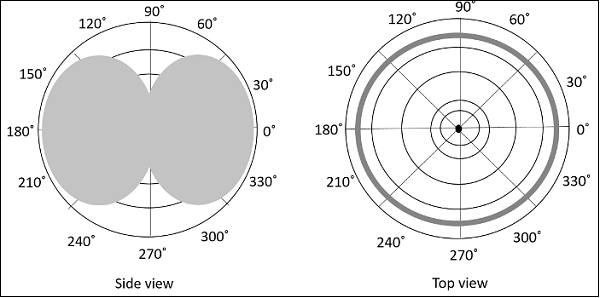
\includegraphics[width=.5\textwidth]{f6.jpg}
    \caption{Dipolo doblado.}
\end{figure}

\newpage
\section{Desarrollo}
Para iniciar con las mediciones se utilizo una antena de dipolo sencillo de onda completa.
\begin{table}[h]
    \centering
    \begin{tabular}{|l|l|l|l|}
    \hline
    Grados & dBm & db & Watts * $1^{-5}$ \\ \hline
    0 & -23 & -53 & 0.5012 \\ \hline
    10 & -25 & -55 & 0.3162 \\ \hline
    20 & -26 & -56 & 0.2512 \\ \hline
    30 & -27 & -57 & 0.1995 \\ \hline
    40 & -30 & -60 & 0.1000 \\ \hline
    50 & -31 & -61 & 0.0794 \\ \hline
    60 & -34 & -64 & 0.0398 \\ \hline
    70 & -36 & -66 & 0.0251 \\ \hline
    80 & -33 & -63 & 0.0501 \\ \hline
    90 & -33 & -63 & 0.0501 \\ \hline
    100 & -34 & -64 & 0.0398 \\ \hline
    110 & -32 & -62 & 0.0631 \\ \hline
    120 & -31 & -61 & 0.0794 \\ \hline
    130 & -29 & -59 & 0.1259 \\ \hline
    140 & -29 & -59 & 0.1259 \\ \hline
    150 & -27 & -57 & 0.1995 \\ \hline
    160 & -27 & -57 & 0.1995 \\ \hline
    170 & -28 & -58 & 0.1585 \\ \hline
    180 & -28 & -58 & 0.1585 \\ \hline
    \end{tabular}
    \caption{Dipolo de onda completa}
    \label{my-label}
\end{table}

\newpage
\subsection{Gráficas de resultados}
\begin{figure}[h]
    \centering
    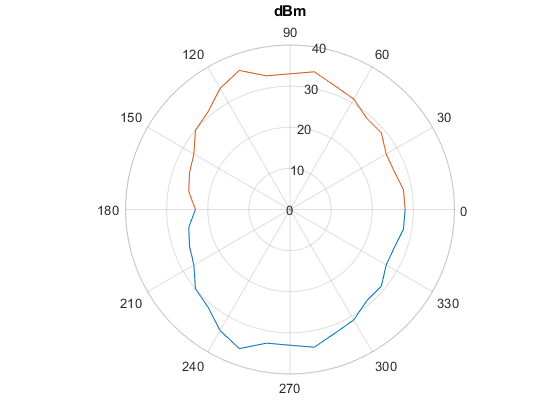
\includegraphics[width=.6\textwidth]{f7.png}
\end{figure}
\begin{figure}[h]
    \centering
    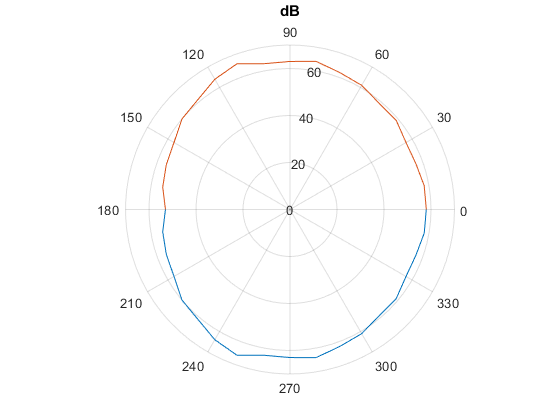
\includegraphics[width=.6\textwidth]{f8.png}
\end{figure}
\begin{figure}[h]
    \centering
    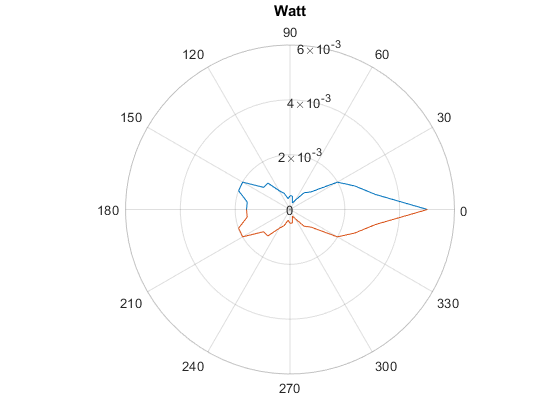
\includegraphics[width=.6\textwidth]{f9.png}
\end{figure}

\newpage
Posteriormente se utilizo una antena de dipolo doblado.
\begin{table}[h]
    \centering
    \begin{tabular}{|l|l|l|l|}
    \hline
    Grados & dBm & db & Watts * $1^{-5}$ \\ \hline
    0 & -29 & -59 & 0.1259 \\ \hline
    10 & -33 & -63 & 0.0501 \\ \hline
    20 & -34 & -64 & 0.0398 \\ \hline
    30 & -36 & -66 & 0.0251 \\ \hline
    40 & -36 & -66 & 0.0251 \\ \hline
    50 & -31 & -61 & 0.0794 \\ \hline
    60 & -31 & -61 & 0.0794 \\ \hline
    70 & -28 & -58 & 0.1585 \\ \hline
    80 & -30 & -60 & 0.1000 \\ \hline
    90 & -27 & -57 & 0.1995 \\ \hline
    100 & -27 & -57 & 0.1995 \\ \hline
    110 & -25 & -55 & 0.3162 \\ \hline
    120 & -27 & -57 & 0.1995 \\ \hline
    130 & -30 & -60 & 0.1000 \\ \hline
    140 & -33 & -63 & 0.0501 \\ \hline
    150 & -37 & -67 & 0.0200 \\ \hline
    160 & -36 & -66 & 0.0251 \\ \hline
    170 & -38 & -68 & 0.0158 \\ \hline
    180 & -30 & -68 & 0.1000 \\ \hline
    \end{tabular}
    \caption{Dipolo de onda completa}
    \label{my-label}
\end{table}
\end{document}